% =====================================================================
% paper/thesis_ch5/sections/methodology.tex
% §5.4 强化学习方法与算法框架（methodology — 共同方法入口）
% =====================================================================
% rev.1（2026-06-17）：§5.4 首版落地。组织遵循"共同骨架 + 带动机的增量"：
%   §5.4.1 部分可观测任务 → 异策略学习问题（POMDP + 在线/离线数据范式）；
%   §5.4.2 异策略 Actor-Critic 共同骨架 + SAC（在线、最大熵分支）；
%   §5.4.3 TD3+BC（确定性 + 单侧行为克隆离线基线）；
%   §5.4.4 ReBRAC-Q（Q 归一化双正则 TD3+BC 变体）；
%   §5.4.5 FQL（流匹配行为建模 + 蒸馏策略）；
%   §5.4.6 训练期特权信息与部署期策略接口（可部署 vs 特权协议）；
%   §5.4.7 实施细节与可复现性（统一符号 + 方法框架总表 + 损失/信息协议汇总表）。
%   公式口径全部对照源码核验：actor/critic loss 与 rebrac.py/td3bc.py/fql.py 一致；
%   ReBRAC-Q critic 侧惩罚采用 a'_D（同轨迹下一步数据动作）口径，非 target smoothing
%   噪声项本身。
%   硬约束守：off-policy→异策略；actor→策略网络(actor)、critic→价值网络(critic)；
%   ReBRAC-Q 首次完整定义为 Q 归一化双正则 TD3+BC 变体，不裸写 ReBRAC 指代本文方法；
%   LayerNorm 写作表征稳定性基础设施（非可选附加能力）；FQL 不以 teacher 为概念主语，
%   改写"流匹配模型积分去噪得到的参考动作 / 蒸馏所得部署策略"；β1/β2 仅作系数含义、
%   不写具体值与优劣；本节不写任何成功率/百分点/排名/负结果/N2'/cross-source 结论，
%   不写"后续节将…"式目录元话语。
%
% rev.2（2026-06-17）：独立对抗复审落地（公式忠实度/红线/语体三视角）。
%   HIGH 删黑话「旋钮」(行114→"显式系数")；正文强调引号统一为弯引号(与 setup.tex 齐)；
%   收尾/铺垫段 forward-looking 言说框架改机制/问题作主语(行26/204)；删空 hedge
%   引导语「需要说明/强调/区分的是」；TD3+BC 系数 α→α_BC 与 α_ent/α_FQL 平行；
%   §5.4.7 补原始动作模仿项求和/均值范数因子说明；FQL 价值网络补"同采层归一化"一句。
%   公式与源码核验通过、§0.4 红线零踩、禁写结果零命中（复审结论）。
% rev.3（2026-06-18）：§5.6 复审配套——章级"检查点选择规则"上提本节（§5.4=算法实现之家）。
%   §5.4.m 增一句：各方法训练内检查点统一按验证成功率/回报/负安全代价/负用时字典序选择，跨种子
%   超参后验选择同此字典序；结果节只补本节特有的后验选择对象。原 td3bc.tex §5.6.m 重复交代收为指针，
%   避免与后续 §5.7/§5.9 实施细节子节重复。其余 §5.4 内容未动。
% 收尾统稿轮（2026-07-08）："沿船体"→"沿机体"（章级术语统一，用户裁定以 setup.tex
%   定义之家为准）；删重复英文括注 ×3（actor/critic/off-policy 首现均在 §5.1/§5.3，
%   §0.5.10 首次括注一次规则）；fig_ch5_method_framework [t]→[tp]（原 [t] 过高无法
%   上版、堵塞 figure 队列致 §5.5 六图漂移节末，F·M2 根因）。零数字/零论证改动。
% rev.4（2026-07-24）：第 4 批 H4 落地——§5.4.1 引入 POMDP 的标准表述原**无 cite**
%   （findings H4 实核项之一），补 \citep{kaelbling1998pomdp}。中英括注不动（首现
%   规则），公式与论证零改动。
% =====================================================================

\section{强化学习方法与算法框架}\label{sec:ch5_methodology}

\S\ref{sec:ch5_setup} 固定了贯穿全章的任务、观测、奖励与数据集协议；本节在此基础上把本章所比较的学习方法纳入同一个强化学习框架。这些方法并非互不相关的算法，而是同一部署约束下对信息的不同利用方式。它们共享策略网络与价值网络的基本分工，共享离线数据或在线交互这两类信息来源，也共享价值自举与行为约束等构件；区别只在于以何种方式把策略约束在数据支持之内，以及在训练阶段允许哪一方接触何种信息。把这些共同构件一次性定义清楚，各方法的机制证据与实验协议便可在共同的算法语言下展开，而不必反复重述算法基础。为此，本节先统一符号、方法边界与共同的异策略 Actor-Critic 骨架，再依次给出在线最大熵方法、行为约束离线基线、双侧正则的离线主线方法、以及以更具表达力的生成式先验为参照目标的离线方法，最后抽象出训练期与部署期的信息协议。

\subsection{从部分可观测任务到异策略学习问题}\label{subsec:ch5_method_pomdp}

\S\ref{subsec:ch5_task} 所述的航行器在尾流场中的运动规划，是一个部分可观测的连续控制问题。真实流场与航行器六自由度动力学的完整状态可记为 $\mathbf{s}_t$，但策略无法直接读取它；策略在每个决策步只能获得由观测算子 $\Omega$ 给出的可部署观测 $\mathbf{o}_t=\Omega(\mathbf{s}_t)$，并据此输出二维连续动作 $\mathbf{a}_t$。沿用部分可观测马尔可夫决策过程（partially observable Markov decision process, POMDP）的标准表述~\citep{kaelbling1998pomdp}，学习目标是寻找一个策略网络 $\pi_\theta$，使其在给定可部署观测下选择的动作能最大化折扣回报：
\begin{equation}
\mathbf{o}_t = \Omega(\mathbf{s}_t),
\qquad
\mathbf{a}_t \sim \pi_\theta(\cdot \mid \mathbf{o}_t),
\qquad
J(\pi_\theta) = \mathbb{E}_{\pi_\theta}\!\left[\sum_{t=0}^{T}\gamma^{t}\, r_t\right],
\label{eq:ch5_pomdp}
\end{equation}
其中 $r_t$ 为 \S\ref{subsec:ch5_reward} 给出的奖励，$\gamma\in(0,1)$ 为折扣因子，$T$ 为回合长度。在确定性策略的情形下，$\pi_\theta(\mathbf{o})$ 直接给出动作而非其分布；本节随方法不同分别采用随机与确定性两类策略网络，但学习目标统一为 \eqref{eq:ch5_pomdp}，并在 \S\ref{subsec:ch5_eval} 的固定评估协议下以任务成功率作为最终度量。这一表述的关键之处在于观测与状态之间的信息落差：策略实际掌握的至多是探针处的局部流速采样，在可部署的 $s_0$ 配置下更只是单点瞬时流速，而真正驱动动力学的是沿机体的等效来流。可部署观测与特权观测之间的这一信息落差，是本章各方法比较的核心所在，其精确定义见 \S\ref{subsec:ch5_obs_deployable} 与 \S\ref{subsec:ch5_obs_privileged}。

策略据以学习的数据来源分为两类，对应在线与离线两种学习范式。在线强化学习允许策略在训练过程中与环境反复交互，把交互产生的转移存入经验回放缓冲区 $\mathcal{B}$，并以此持续评估与改进当前策略。离线强化学习则不进行任何在线交互，策略只能使用一个预先采集、训练期间固定不变的数据集
\begin{equation}
\mathcal{D} = \big\{\,(\mathbf{o}_t,\ \mathbf{a}_t,\ r_t,\ \mathbf{o}_{t+1},\ e_t)\,\big\},
\label{eq:ch5_offline_data}
\end{equation}
其中 $e_t$ 为终止标志，数据由若干行为策略按 \S\ref{subsec:ch5_datasets} 的协议采集。两种范式共享同一套观测、动作与奖励定义，但离线范式带来一处本质困难：策略改进的方向由价值网络的估计引导，而价值网络只在数据覆盖到的状态–动作区域内可靠，一旦策略偏离数据支持去查询分布外动作（out-of-distribution action），价值估计便会外推并产生系统性高估，进而把策略推向数据从未验证的区域，形成自我强化的偏差~\citep{levine2020offline}。因此离线方法的共同任务，是在尽量改进策略的同时把它约束在数据支持之内；本节后续介绍的三种离线方法，差别正在于以何种形式施加这一约束。

\subsection{异策略 Actor-Critic 共同骨架与在线方法 SAC}\label{subsec:ch5_method_sac}

本章所用的学习方法都属于异策略 Actor-Critic 框架。该框架把学习分解为两个相互耦合的部分：策略网络负责在给定观测下产生动作，价值网络则估计动作价值函数 $Q(\mathbf{o},\mathbf{a})$，即在该观测下执行该动作并此后遵循当前策略所能获得的期望折扣回报。异策略意味着用于更新的转移不必来自当前策略本身，既可以是回放缓冲区中由历史策略产生的交互，也可以是离线数据集中由行为策略采集的轨迹；这一性质使同一框架既能支撑在线学习，也能支撑从固定数据集的离线学习。价值网络通过自举（bootstrap）更新：以单步奖励加上对后继观测的价值估计构成回归目标 $y$，并令价值网络逼近该目标，
\begin{equation}
y = r + \gamma\,(1-e)\,\min_{j=1,2} Q_{\bar\phi_j}(\mathbf{o}',\mathbf{a}'),
\qquad
\mathcal{L}_{Q} = \sum_{j=1,2}\mathbb{E}\big[\big(Q_{\phi_j}(\mathbf{o},\mathbf{a}) - y\big)^2\big].
\label{eq:ch5_critic_target}
\end{equation}
其中 $\bar\phi_j$ 为价值网络的目标网络参数，随主网络以系数 $\tau$ 作软更新。为抑制价值高估，框架采用两套价值网络并在目标中取二者较小值（clipped double-Q）；$\mathbf{a}'$ 为后继观测下由策略选取的动作，其具体形式随方法而异，是区分各方法的首要接口。

后继动作 $\mathbf{a}'$ 的选取方式区分出两个分支。随机策略分支以一个随机策略网络刻画动作分布，并在自举目标中加入策略熵；确定性策略分支则使用确定性策略网络，并借助目标策略平滑与延迟策略更新来稳定训练——后继动作由目标策略的输出叠加一段经截断的高斯噪声给出，
\begin{equation}
\tilde{\mathbf{a}}' = \mathrm{clip}\big(\pi_{\bar\theta}(\mathbf{o}') + \epsilon,\ -1,\ 1\big),
\qquad
\epsilon \sim \mathrm{clip}\big(\mathcal{N}(0,\sigma^2 I),\ -c,\ c\big),
\label{eq:ch5_target_smoothing}
\end{equation}
其中 $\pi_{\bar\theta}$ 为目标策略网络，$\sigma$ 与 $c$ 分别为平滑噪声的标准差与截断幅度。双价值网络、目标网络、目标策略平滑与延迟策略更新，是 TD3 一系确定性方法用于减轻价值高估与训练震荡的共同基础设施~\citep{fujimoto2018td3}；本章的三种离线方法都建立在这一确定性分支之上，其差异在后续小节给出。

在线情形采用最大熵异策略方法 SAC~\citep{haarnoja2018sac}。SAC 属随机策略分支，以一个经压缩高斯分布参数化的策略网络刻画动作分布，并在优化回报的同时最大化策略熵，从而在探索与利用之间取得平衡。其自举目标在 \eqref{eq:ch5_critic_target} 的基础上对后继动作的对数概率加以惩罚，策略改进则在价值与熵之间权衡，
\begin{equation}
\mathcal{L}_{\pi}^{\mathrm{SAC}}
= \mathbb{E}_{\mathbf{o}\sim\mathcal{B},\ \mathbf{a}\sim\pi_\theta}
\big[\,\alpha_{\mathrm{ent}}\log\pi_\theta(\mathbf{a}\mid\mathbf{o}) - Q_\phi(\mathbf{o},\mathbf{a})\,\big],
\label{eq:ch5_sac_actor}
\end{equation}
其中熵温度系数 $\alpha_{\mathrm{ent}}$ 在训练中自动调节，以维持目标熵水平。在本章中，SAC 承担两个方法性角色。一个角色是在线情形下任务可学习性的参照，用以考察策略能否仅凭可部署观测在交互中习得有效的运动规划；另一个角色是离线数据的一类来源，即由 SAC 训练轨迹不同阶段的检查点构成质量递增的采集器（\S\ref{subsec:ch5_datasets}）。这两个角色都不要求 SAC 在部署性能上与离线方法竞争，它在本章中并非主线算法，而是为离线比较提供在线一侧的参照与数据。

\subsection{行为约束离线 Actor-Critic：TD3+BC}\label{subsec:ch5_method_td3bc}

在确定性分支上施加行为约束的最简形式是 TD3+BC~\citep{fujimoto2021td3bc}。它在 TD3 的确定性策略梯度之上叠加一项行为克隆（behavior cloning, BC）惩罚，使策略在追求高价值动作的同时不至于偏离数据集中实际出现过的动作。其价值网络按 \eqref{eq:ch5_critic_target} 与 \eqref{eq:ch5_target_smoothing} 给出的确定性自举目标更新，不含任何附加惩罚项；行为约束只作用于策略改进一侧，
\begin{equation}
\mathcal{L}_{\pi}^{\mathrm{TD3{+}BC}}
= -\,\lambda_{\mathrm{TD3{+}BC}}\,
\mathbb{E}_{\mathbf{o}\sim\mathcal{D}}\,Q_\phi\big(\mathbf{o},\pi_\theta(\mathbf{o})\big)
+ \mathbb{E}_{(\mathbf{o},\mathbf{a})\sim\mathcal{D}}\,\big\|\pi_\theta(\mathbf{o}) - \mathbf{a}\big\|^2,
\qquad
\lambda_{\mathrm{TD3{+}BC}}
= \frac{\alpha_{\mathrm{BC}}}{\mathbb{E}\,\big|Q_\phi(\mathbf{o},\pi_\theta(\mathbf{o}))\big|}.
\label{eq:ch5_td3bc_actor}
\end{equation}
第一项推动策略选择价值更高的动作，第二项把策略输出拉向同一观测下的数据动作 $\mathbf{a}$。系数 $\lambda_{\mathrm{TD3{+}BC}}$ 按批量内价值幅度的均值对价值项作归一化，使其量级与行为克隆项可比，从而单一超参数 $\alpha_{\mathrm{BC}}$ 即可在不同奖励尺度的数据集上一致地调节“改进”与“模仿”之间的权衡。这一设计把离线策略改进约束在数据支持附近，是异策略离线学习中行为约束的基准形式。

TD3+BC 给出了行为约束离线方法的最小实现，但它把数据支持的全部信息压缩在单一的原始动作模仿项上。这一项无法区分数据中行为质量、动作噪声与价值外推这几类不同来源的影响：当数据动作本身质量参差或带有噪声时，对原始动作的逐点模仿会把噪声一并学入策略；而仅靠策略一侧的约束，也不足以阻止价值网络在自举链路上对分布外的后继动作产生外推偏差。这些局限提示，更充分的离线方法需要在策略与价值两侧同时施加约束，或为模仿提供比原始数据动作更可靠的参照目标。本章后续的两种离线方法分别沿这两个方向展开，而 TD3+BC 则作为它们的共同参照基线。

\subsection{ReBRAC-Q：Q 归一化双正则 TD3+BC 变体}\label{subsec:ch5_method_rebrac}

本章的离线主线方法记为 ReBRAC-Q，它是一个 Q 归一化的双侧正则 TD3+BC 变体。它沿用 TD3+BC 以批量价值幅度对策略改进项作归一化的做法（下称 Q 归一化），并在此基础上把行为约束从策略一侧扩展到策略与价值两侧：策略一侧仍以原始动作行为克隆把策略拉向数据动作，价值一侧则在自举目标中额外惩罚后继动作对数据支持的偏离。这一双侧正则的设计源自最小改动型的离线方法 ReBRAC~\citep{tarasov2023rebrac}；本文方法与原始 ReBRAC 的主要差异，在于策略改进项是否采用 TD3+BC 风格的批量均值 $|Q|$ 归一化~\citep{fujimoto2021td3bc}——本文方法采用这一归一化，故以 ReBRAC-Q 命名，全章统一使用该名称指代本文的离线主线方法。

策略一侧的目标在 TD3+BC 的形式上把行为克隆项的强度显式参数化。记策略改进项的归一化系数为 $\lambda_Q$，由批量内价值幅度的均值（取自当前策略动作处、并在该系数计算中切断梯度）给出，
\begin{equation}
\bar Q = \mathbb{E}_{\mathbf{o}\sim\mathcal{D}}\,\big|Q_\phi(\mathbf{o},\pi_\theta(\mathbf{o}))\big|_{\mathrm{detach}},
\qquad
\lambda_Q = \frac{1}{\max(\bar Q,\ \varepsilon)},
\label{eq:ch5_rebrac_qnorm}
\end{equation}
策略目标则为归一化的价值改进项与原始动作行为克隆项之和，
\begin{equation}
\mathcal{L}_{\pi}^{\mathrm{ReBRAC\text{-}Q}}
= -\,\lambda_Q\,
\mathbb{E}_{\mathbf{o}\sim\mathcal{D}}\,Q_\phi\big(\mathbf{o},\pi_\theta(\mathbf{o})\big)
+ \beta_1\,
\mathbb{E}_{(\mathbf{o},\mathbf{a})\sim\mathcal{D}}\,\big\|\pi_\theta(\mathbf{o}) - \mathbf{a}\big\|^2.
\label{eq:ch5_rebrac_actor}
\end{equation}
系数 $\beta_1$ 控制策略输出贴近数据动作的强度，是策略一侧行为约束强度的显式系数；$\lambda_Q$ 只对价值项作尺度归一化（$\varepsilon$ 为防止除零的数值下界），并不改变奖励定义或任务目标。$\beta_1$ 与 TD3+BC 中的 $\alpha_{\mathrm{BC}}$ 只有在本文这一 Q 归一化写法下才存在近似的换算关系，二者并非同一量纲下的同一系数；本节只给出系数含义，其取值与跨设定的对照留待相应结果节讨论。

价值一侧的正则项作用于自举目标。沿用 \eqref{eq:ch5_target_smoothing} 给出的经目标平滑的后继动作 $\tilde{\mathbf{a}}'$，ReBRAC-Q 在 \eqref{eq:ch5_critic_target} 的双价值网络目标基础上，对后继动作偏离数据支持的程度施加二次惩罚，
\begin{equation}
y^{\mathrm{ReBRAC\text{-}Q}}
= r + \gamma\,(1-e)\Big[\,
\min_{j=1,2} Q_{\bar\phi_j}(\mathbf{o}',\tilde{\mathbf{a}}')
- \beta_2\,\big\|\tilde{\mathbf{a}}' - \mathbf{a}'_{\mathcal D}\big\|^2
\,\Big],
\label{eq:ch5_rebrac_target}
\end{equation}
其中 $\mathbf{a}'_{\mathcal D}$ 是同一条离线轨迹中与 $\mathbf{o}'$ 对应的下一步数据动作。该惩罚比较的是自举所用的后继动作 $\tilde{\mathbf{a}}'$ 与数据中实际记录的下一步动作 $\mathbf{a}'_{\mathcal D}$ 之间的偏离，因而衡量的是价值自举是否落在数据支持之内——当目标动作偏离数据动作越远，价值目标被压低得越多，从而抑制价值网络沿自举链路对分布外动作的外推。系数 $\beta_2$ 控制这一价值侧约束的强度。它与策略一侧的行为克隆项作用机理不同：策略侧的项约束的是部署时实际执行的策略输出，价值侧的项约束的则是训练中价值目标所依赖的后继动作；两者共同把策略与价值都锚定在数据分布附近，是 ReBRAC-Q 区别于单侧约束 TD3+BC 的核心增量。

ReBRAC-Q 还在价值网络中引入层归一化（LayerNorm）作为表征稳定性的基础设施。离线价值估计长期在固定数据集上自举，价值网络的内部表征容易随训练发散，进而放大上述外推偏差；在价值网络中加入层归一化可约束其内部激活的尺度，与上述双侧行为约束共同维持离线价值估计的稳定。层归一化既不是部署阶段的额外信息，也不是任何额外的传感能力，它与“特权信息是否必需”这一问题相互正交：它服务于价值估计在训练期的数值稳定，而不改变策略在部署时所依赖的观测。因此本章把层归一化视为离线价值学习的必要构件，而非可有可无的附加项。

\subsection{FQL：流匹配行为建模与蒸馏策略}\label{subsec:ch5_method_fql}

ReBRAC-Q 以原始数据动作作为模仿目标，这在数据动作可靠时是恰当的，但当行为分布呈多模态或带有噪声时，对原始动作的逐点模仿未必给出最好的参照。FQL~\citep{park2025fql} 沿另一方向改造行为约束：它不直接以原始数据动作为模仿目标，而是先用一个生成式模型刻画数据中的行为分布，再以该模型给出的参照动作引导策略。具体而言，FQL 把条件动作分布建模为从高斯噪声到数据动作的连续流（流匹配，flow-matching），并学习一个条件速度场 $v_\eta(\mathbf{x}_t,t\mid\mathbf{o})$；沿噪声到数据动作的线性插值路径，速度场的回归目标恰为数据动作与噪声之差，
\begin{equation}
\mathbf{x}_t = (1-t)\,\mathbf{x}_0 + t\,\mathbf{a},
\quad \mathbf{x}_0 \sim \mathcal{N}(0,I),
\quad v^\star = \mathbf{a} - \mathbf{x}_0,
\qquad
\mathcal{L}_{\mathrm{flow}}
= \mathbb{E}\,\big\|v_\eta(\mathbf{x}_t,t\mid\mathbf{o}) - v^\star\big\|^2,
\label{eq:ch5_fql_flow}
\end{equation}
其中 $t\in[0,1]$ 为流时间，$\mathbf{x}_t$ 为该路径上的中间点。沿学得的速度场对噪声起点作积分，即可得到一个经去噪的参照动作，记为 $\mathbf{a}_{\mathrm{FM}}(\mathbf{o})$，它代表在该观测下行为分布所支持的一个高似然动作。

部署阶段并不直接执行上述生成式模型的积分过程，而是执行一个一步确定性策略网络 $\mu_\theta$。该策略网络通过蒸馏对齐到流匹配模型积分得到的参照动作 $\mathbf{a}_{\mathrm{FM}}$，同时仍借助价值网络以归一化的价值改进项进行策略改进，
\begin{equation}
\mathbf{a}_{\mathrm{FM}}(\mathbf{o}) = \mathrm{Integrate}\big(v_\eta(\cdot,\cdot\mid\mathbf{o})\big),
\qquad
\mathcal{L}_{\pi}^{\mathrm{FQL}}
= -\,\lambda_Q\,\mathbb{E}\,Q_\phi\big(\mathbf{o},\mu_\theta(\mathbf{o})\big)
+ \alpha_{\mathrm{FQL}}\,\mathbb{E}\,\big\|\mu_\theta(\mathbf{o}) - \mathbf{a}_{\mathrm{FM}}(\mathbf{o})\big\|^2,
\label{eq:ch5_fql_actor}
\end{equation}
其价值网络按确定性自举目标更新，不含价值一侧的行为克隆惩罚；与 ReBRAC-Q 相同，其价值网络亦采用层归一化以稳定离线价值估计。FQL 与 ReBRAC-Q 在框架上高度一致：二者都属确定性策略分支，都以 Q 归一化的价值改进项驱动策略，都通过一项二次模仿项把策略约束在数据分布附近。二者的关键差异在于模仿项所指向的参照目标——ReBRAC-Q 指向原始数据动作 $\mathbf{a}$，FQL 指向由流匹配模型去噪生成的参照动作 $\mathbf{a}_{\mathrm{FM}}$。参照目标来源上的这一差异，正是本章在算法与数据条件之间作交互分析时所依据的方法接口。

\subsection{训练期特权信息与部署期策略接口}\label{subsec:ch5_method_protocol}

上述方法都在同一部署接口下学习，但在训练阶段允许价值网络接触的信息可以不同。\S\ref{subsec:ch5_obs_privileged} 已据此定义了可部署协议与特权协议：前者的策略网络与价值网络都只读可部署观测 $\mathbf{o}_t$，后者的价值网络在训练期额外读取特权观测 $\mathbf{o}_t^{\mathrm{priv}}$、而策略网络始终只读 $\mathbf{o}_t$。这一非对称安排沿用非对称 Actor-Critic 的思路~\citep{pinto2017asymmetric}，让价值网络在训练期借助更完整的信息给出更准确的价值估计，同时保持策略本身可部署；同样的安排亦可施加于在线 SAC，其价值网络在训练期可选地读取特权观测，构成在线情形下的特权消融对照。在算法记号上，本节所列价值网络目标式（如~\eqref{eq:ch5_critic_target} 与~\eqref{eq:ch5_rebrac_target}）均按可部署协议写出，价值网络只读 $\mathbf{o}$；在特权协议下，相应价值网络及其目标网络改读 $Q_\phi(\mathbf{o},\mathbf{a},\mathbf{o}^{\mathrm{priv}})$ 与 $Q_{\bar\phi_j}(\mathbf{o}',\cdot\,,\mathbf{o}'^{\mathrm{priv}})$，其余形式不变。

如 \S\ref{subsec:ch5_obs_privileged} 所述，两种协议的部署接口完全相同：评估与部署阶段只执行策略网络，价值网络被弃用，特权观测不入执行回路，故所得策略在部署时都只依赖单点局部流速。于是特权协议相对可部署协议唯一改变的，是训练期价值网络可用的信息量；这使二者构成一组干净的对照，可单独考察在训练期把特权信息提供给价值网络是否会改变所得可部署策略的性能。需与之区分的是，这里的特权观测是仅供价值网络读取的训练期信号，改变的是价值估计所依据的信息，而非 \S\ref{subsec:ch5_datasets} 中那种通过读取全场流场提升离线数据来源与质量的行为采集器。

\subsection{实施细节与可复现性}\label{subsec:ch5_method_impl}

本章各方法共用一套符号与实现口径。状态、观测、动作、奖励、终止与后继观测分别记为 $\mathbf{s}_t$、$\mathbf{o}_t$、$\mathbf{a}_t$、$r_t$、$e_t$ 与 $\mathbf{o}_{t+1}$，离线数据集记为 $\mathcal{D}$、在线回放缓冲区记为 $\mathcal{B}$，策略网络与价值网络分别记为 $\pi_\theta$（确定性情形下亦记为 $\mu_\theta$）与 $Q_\phi$，其目标网络参数记为 $\bar\theta,\bar\phi_j$，折扣因子与软更新系数分别为 $\gamma$ 与 $\tau$。终止标志记为 $e_t\in\{0,1\}$，以区别于 \S\ref{sec:ch5_setup} 中表示到目标距离的 $d$；环境层的偏航率 $r$（本体状态分量，区别于奖励 $r_t$）、速度比 $\lambda$ 等量亦沿用 \S\ref{sec:ch5_setup} 的记号，本节不再重复。后继观测下用于自举的动作记为 $\mathbf{a}'$，其经目标策略平滑的形式记为 $\tilde{\mathbf{a}}'$，同一离线轨迹中与后继观测 $\mathbf{o}'$ 对应的下一步数据动作记为 $\mathbf{a}'_{\mathcal D}$。行为约束系数中，$\alpha_{\mathrm{BC}}$ 为 TD3+BC 的单一行为克隆权重，$\beta_1,\beta_2$ 分别为 ReBRAC-Q 策略一侧与价值一侧的行为约束权重，$\alpha_{\mathrm{FQL}}$ 为 FQL 的蒸馏模仿权重，$\alpha_{\mathrm{ent}}$ 为 SAC 的熵温度系数。各方法的二次模仿与支持惩罚项（含策略一侧的原始动作模仿与价值一侧的下一步支持惩罚）在实现上或按动作维求和、或按动作维取均值，二者相差一个与动作维数有关的常数因子，已并入相应的行为约束系数，不影响其作为强度调节量的含义。Q 归一化中的下界 $\varepsilon$ 仅为数值稳定而设，不承担任何调节作用。确定性分支共用的目标策略平滑噪声、噪声截断幅度与延迟策略更新频率，作为 TD3 一系方法的共同实现口径，在各离线方法中保持一致；其中 TD3+BC 的策略改进项按其原始实现取单一价值网络的估计；其余方法（SAC、ReBRAC-Q 与 FQL）的策略改进项，以及所有方法的自举目标，均取双价值网络的较小值。各式中出现于策略改进项的 $Q_\phi$ 均按此约定理解。特权观测的维度与物理含义已在 \S\ref{subsec:ch5_obs_privileged} 给定，本节不再重复其推导；离线数据集为支持特权协议，随每条转移一并记录特权观测及其后继（\S\ref{subsec:ch5_impl}）。各方法训练内的检查点统一按验证集上的成功率、回报、负安全代价与负用时的字典序选择；需作跨随机种子的超参数后验选择时，亦按相应验证指标的同一字典序进行，以避免人工挑选检查点或事后口径漂移，各结果节只补充本节特有的后验选择对象。各方法的具体超参数取值、数据集规模与统计结果，随相应结果节给出。

图~\ref{fig:ch5_method_framework} 给出四种方法的统一框架与派生关系；表~\ref{tab:ch5_method_framework} 汇总四种方法在训练范式、策略输出、行为约束与本章角色上的坐标，表~\ref{tab:ch5_method_loss} 进一步给出各方法的策略目标、价值目标、模仿参照对象，以及价值网络在各协议下可读的观测与特权信息可能出现的位置。两表统一了后续结果节所引用的符号与方法关系：异策略 Actor-Critic 是四种方法的共同框架，SAC 与三种离线方法的区别在于随机与确定性策略以及在线与离线数据来源，三种离线方法之间的区别则集中在行为约束的位置（策略侧、价值侧）、参照目标的来源（原始数据动作、流匹配参照动作）与价值表征稳定性构件上。这些差异都不改变策略在部署时只读取单点局部观测这一共同接口，因而后续各节对它们的比较，都建立在同一组符号与同一套部署约束之上。

\begin{figure}[tp]
    \centering
    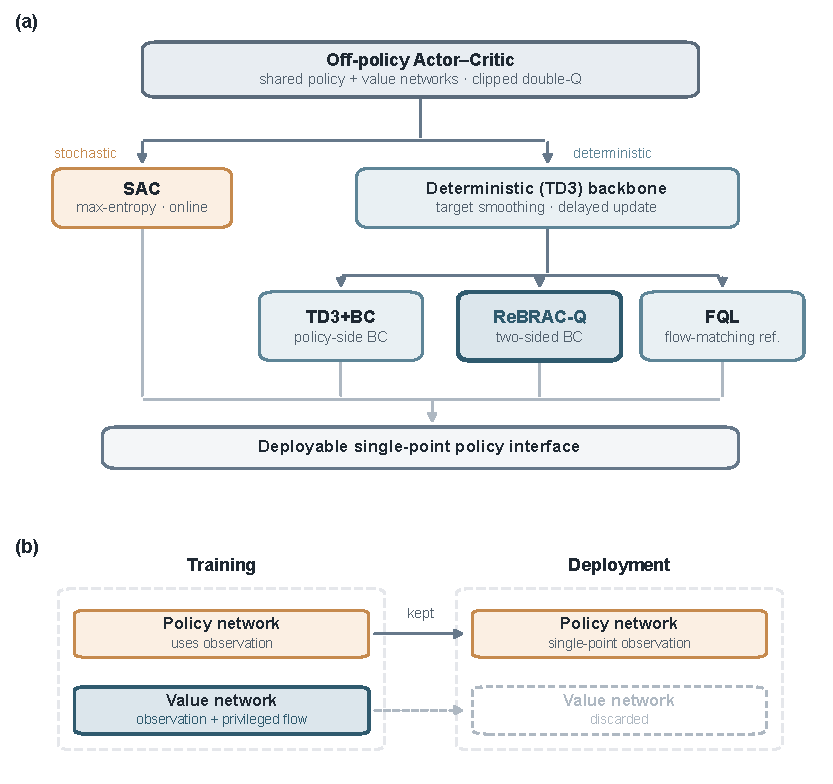
\includegraphics[width=138mm]{figures/fig_ch5_method_framework.pdf}
    \caption{本章方法的统一框架与派生关系（图中不含任何性能数值）。(a) 四种方法共享异策略 Actor--Critic 骨架（策略网络与价值网络、截断双 $Q$ 自举）；由此分出随机策略分支（SAC，在线最大熵）与确定性（TD3）分支，后者派生出三种行为约束离线方法——TD3+BC（仅策略侧行为克隆）、ReBRAC-Q（策略与价值双侧行为克隆，深色框为本章离线主线）与 FQL（以流匹配参照动作为模仿目标）；四者在部署期收敛到同一单点可部署策略接口。ReBRAC-Q 与 FQL 的价值网络均采用层归一化（\S\ref{subsec:ch5_method_rebrac}、\S\ref{subsec:ch5_method_fql}），图中未单列。(b) 训练期与部署期的信息协议：策略网络始终只读可部署观测；价值网络在特权协议下训练时额外读取特权流速 $\mathbf{o}^{\mathrm{priv}}$，部署阶段价值网络被弃用、特权信息消失，故部署传感与训练所用协议无关。各方法的策略目标与价值目标见 \S\ref{subsec:ch5_method_sac}--\S\ref{subsec:ch5_method_fql} 及表~\ref{tab:ch5_method_loss}。}
    \label{fig:ch5_method_framework}
\end{figure}

\begin{table}[t]
\centering
\caption{本章强化学习方法框架总表。四种方法同属异策略 Actor-Critic 框架，差异集中在策略形式与行为约束；四者的策略网络在两协议下均只读可部署观测，价值网络在各方法与协议下可读的观测、以及特权信息可能出现的位置见表~\ref{tab:ch5_method_loss}。“本章角色”列只标方法定位，不含结果结论；层归一化是 ReBRAC-Q 价值网络的表征稳定性构件，归入其行为约束/先验栏。}
\label{tab:ch5_method_framework}
\setlength{\tabcolsep}{4pt}
\begin{tabular}{l l l >{\raggedright\arraybackslash}p{0.30\linewidth} >{\raggedright\arraybackslash}p{0.22\linewidth}}
\toprule
\textbf{方法} & \textbf{范式} & \textbf{策略输出} & \textbf{行为约束 / 先验} & \textbf{本章方法角色} \\
\midrule
SAC & 在线 & 随机策略（最大熵） & 熵正则 & 在线可学性参照与数据采集 \\
TD3+BC & 离线 & 确定性策略 & 原始动作行为克隆 & 离线基线 \\
ReBRAC-Q & 离线 & 确定性策略 & 策略与价值双侧行为克隆，含 Q 归一化与层归一化 & 离线主线 \\
FQL & 离线 & 蒸馏确定性策略 & 流匹配参照动作 & 算法—数据条件交互对照 \\
\bottomrule
\end{tabular}
\end{table}

\begin{table}[t]
\centering
\caption{本章方法的损失函数与信息协议汇总。各方法共用 \eqref{eq:ch5_critic_target} 的双价值网络自举与 \eqref{eq:ch5_target_smoothing} 的确定性目标平滑（SAC 为其随机最大熵变体）；ReBRAC-Q 在价值目标中额外含 $\beta_2$ 的下一步支持惩罚。“特权信息可能出现处”指特权观测在该方法中可被读取的网络，部署阶段一律不出现。}
\label{tab:ch5_method_loss}
\setlength{\tabcolsep}{4pt}
\begin{tabular}{l >{\raggedright\arraybackslash}p{0.26\linewidth} >{\raggedright\arraybackslash}p{0.18\linewidth} >{\raggedright\arraybackslash}p{0.17\linewidth} >{\raggedright\arraybackslash}p{0.15\linewidth}}
\toprule
\textbf{方法} & \textbf{策略目标} & \textbf{价值目标} & \textbf{模仿 / 参照对象} & \textbf{特权信息可能出现处} \\
\midrule
SAC & 熵正则策略改进~\eqref{eq:ch5_sac_actor} & 软 Bellman 目标 & 无显式行为克隆项 & 价值网络（在线特权消融，可选） \\
TD3+BC & Q 归一化策略改进与原始动作行为克隆~\eqref{eq:ch5_td3bc_actor} & TD3 自举目标~\eqref{eq:ch5_critic_target} & 数据动作 $\mathbf{a}$ & 价值网络（两协议均可） \\
ReBRAC-Q & Q 归一化策略改进与 $\beta_1$ 原始动作行为克隆~\eqref{eq:ch5_rebrac_actor} & 含 $\beta_2$ 下一步支持惩罚的 TD 目标~\eqref{eq:ch5_rebrac_target} & 数据动作 $\mathbf{a}$（策略侧）、$\mathbf{a}'_{\mathcal D}$（价值侧） & 价值网络（两协议均可） \\
FQL & Q 归一化策略改进与蒸馏参照行为克隆~\eqref{eq:ch5_fql_actor} & TD 式自举目标 & 流匹配参照动作 $\mathbf{a}_{\mathrm{FM}}$ & 本章 FQL 线不依赖 \\
\bottomrule
\end{tabular}
\end{table}

在上述统一框架下，各方法的差异被归结为三类接口选择：行为约束施加的位置、模仿所依据的参照目标的来源，以及训练期价值网络可接触的信息边界。正因如此，后续各节对在线方法、行为约束离线基线、双侧正则离线主线方法与生成式先验离线方法的比较，落在同一组符号与同一套部署约束之内，成为关于“在固定部署接口下如何利用既有信息与数据”这一核心问题的可相互参照的考察，而非互不相干的算法堆叠。

% 本节一图两表：在进入 §5.5 前冲刷 §5.4 的浮动体，避免其漂入下一节正文
% （与 online.tex 节末同一做法）。第 4 批新增文本使 §5.5 正文提前起页，
% 三个浮动一度落到 §5.5 页面内、距首引超两页（收尾统稿轮包 B 治过的同一形态）。
\clearpage
